%!TEX encoding = utf8
%!TeX spellcheck = en_GB
%%%%%%%%%%%%%%%%%%%%%%%%%%%%%%%%%%%%%%%%%%%%%%%%%%%%%%%%%%%%%%%%%%
\documentclass{thesis}

\chapter{Introduction}

  During the third lab session the control has been fixed and refined and the power readings Simulink submodule has been added. The following is a brief summary of the work carried out on this third session. The final results of this lab sessions will be presented on the final report.\\

  \begin{figure}[H]
    \centering
    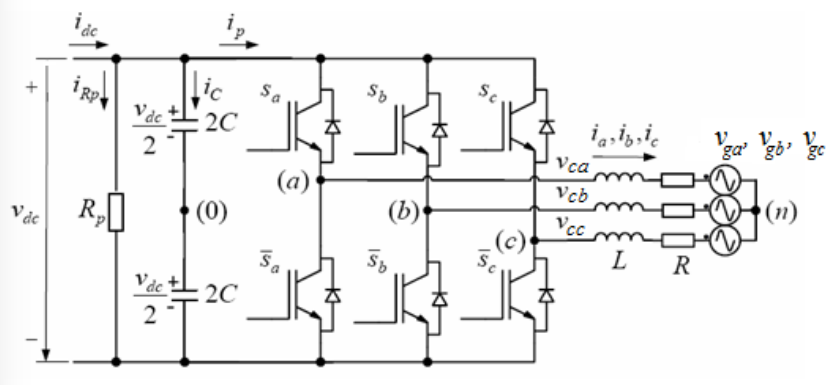
\includegraphics[width=.8\linewidth]{Images/FullConvFig.png}
    \caption{Three-phase inverter connected to the grid}
    \label{ModelFig}
  \end{figure}

  \begin{figure}[H]
    \centering
    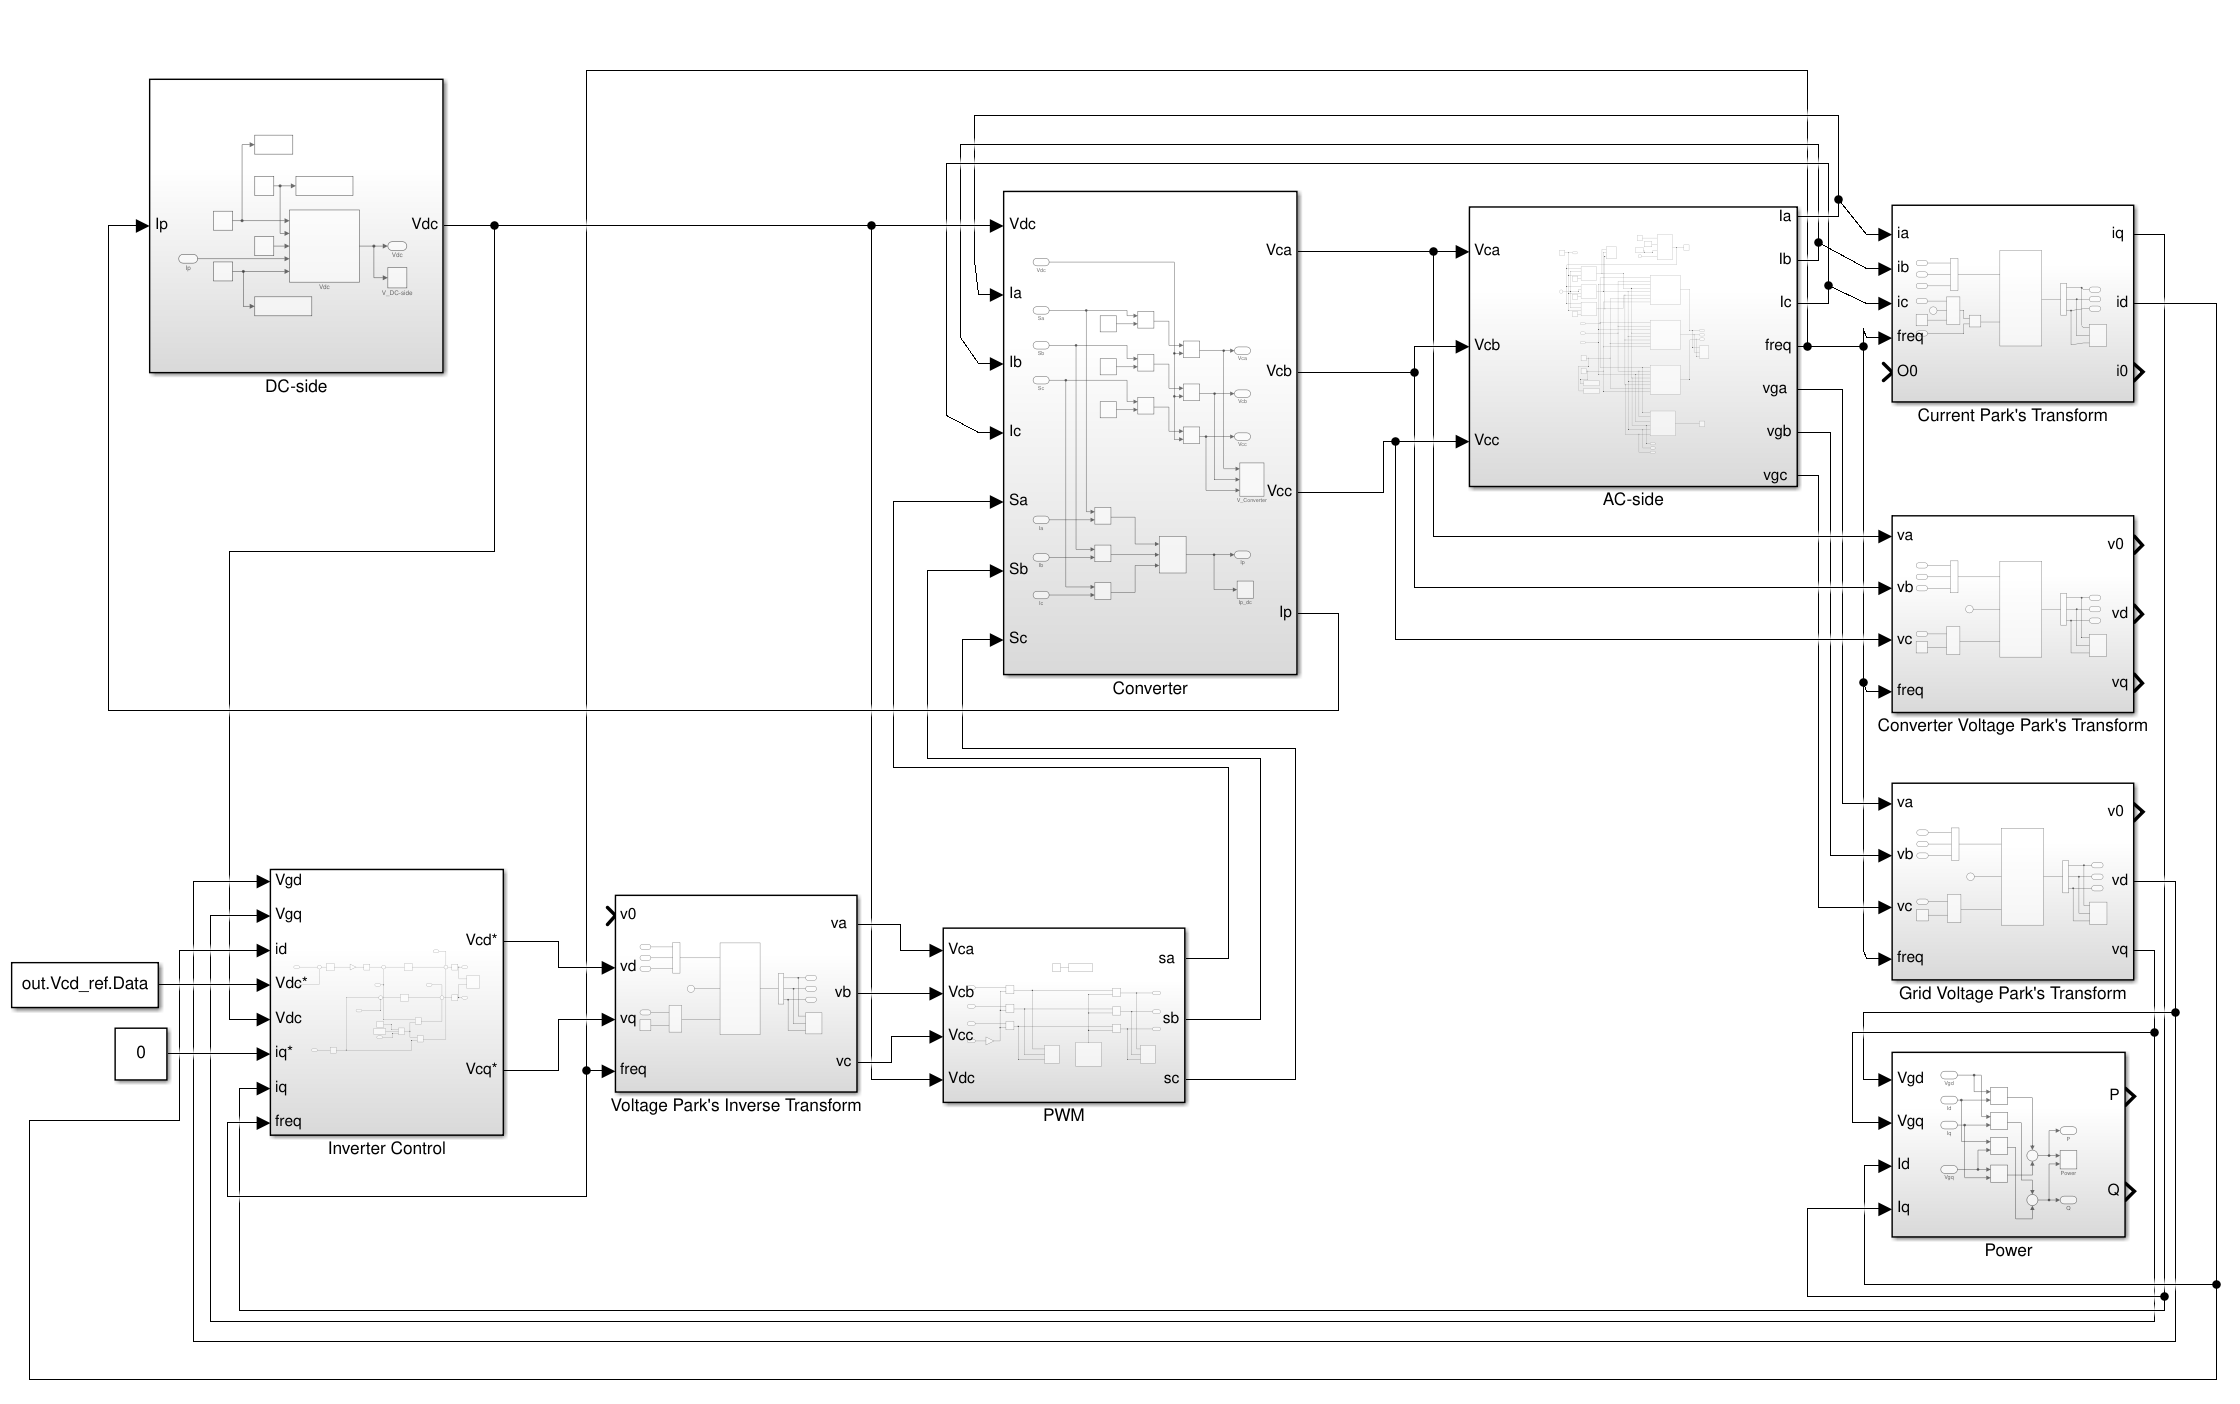
\includegraphics[width=.8\linewidth]{Images/FinalResult.png}
    \caption{Final model after the third lab session}
    \label{S3Model}
  \end{figure}


\chapter{Fixing and tuning the control}

  One of the more important parts of this session was to debug the control. PI constants aside, the biggest problem I was facing was related to the sample time of the simulation, which was set to auto meaning that the model would go out of control due to an uncontrolled time step. This does not mean I changed the converter's frequency to get better results, but I changed the simulation parameters so that the model can run with less error. However this change implies the simulation is now much more expensive in terms of computing in exchange for accuracy.\\

  The following is a comparison with no changes to the model, constants or otherwise, of the impact the simulation sample time has on its results.

  \begin{figure}[H]
      \centering
      \subfloat[Sample time: 1e-4s]{{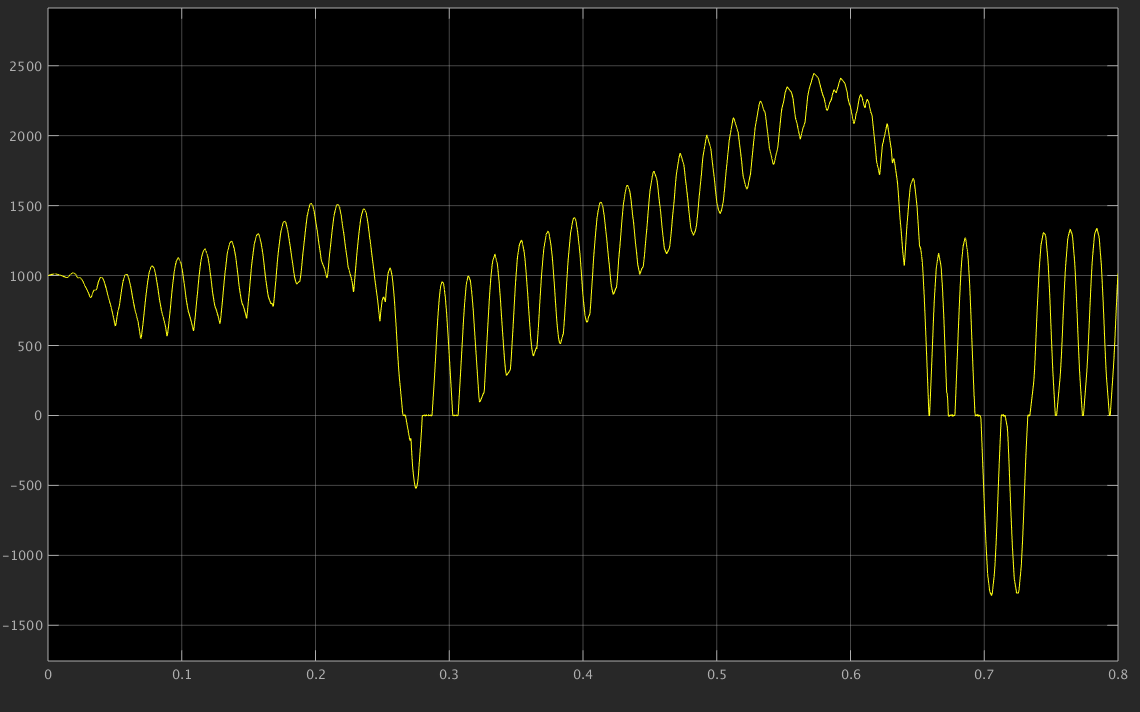
\includegraphics[width=.45\linewidth]{Images/bad1e4Sample_V_DC-side.png} }}%
      \qquad
      \subfloat[Sample time: 1e-5s]{{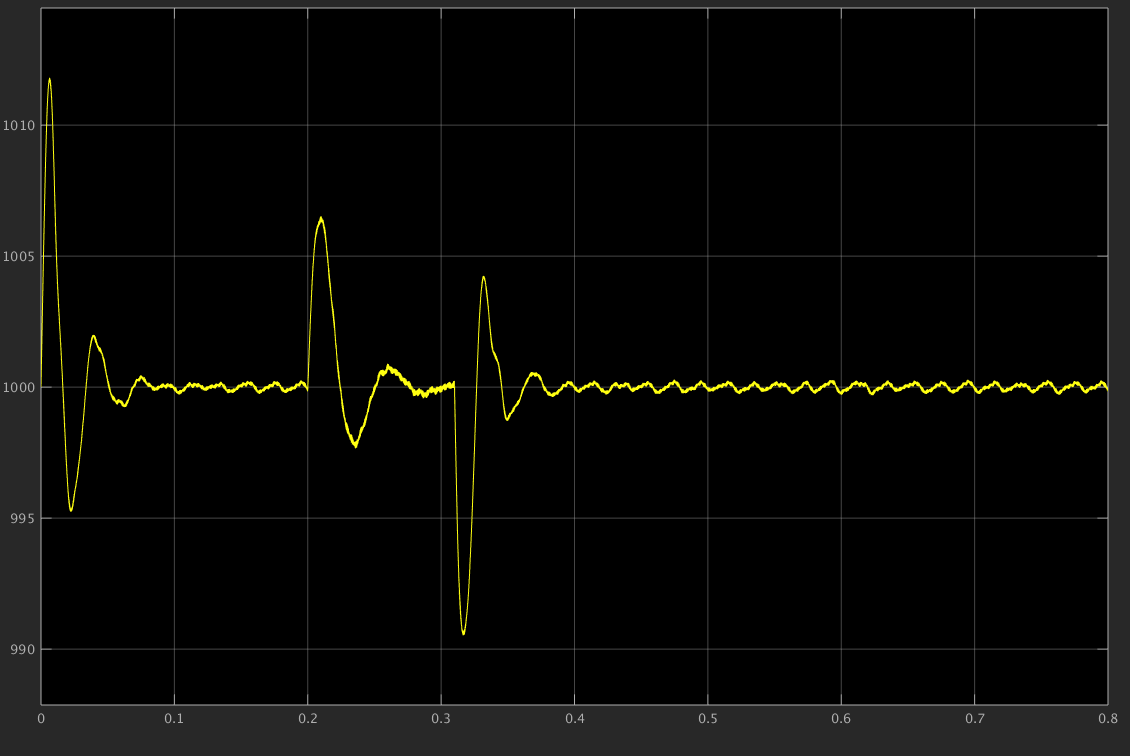
\includegraphics[width=.45\linewidth]{Images/bad1e5Sample_V_DC-side.png} }}%

      \centering
      \subfloat[Sample time: 1e-6s]{{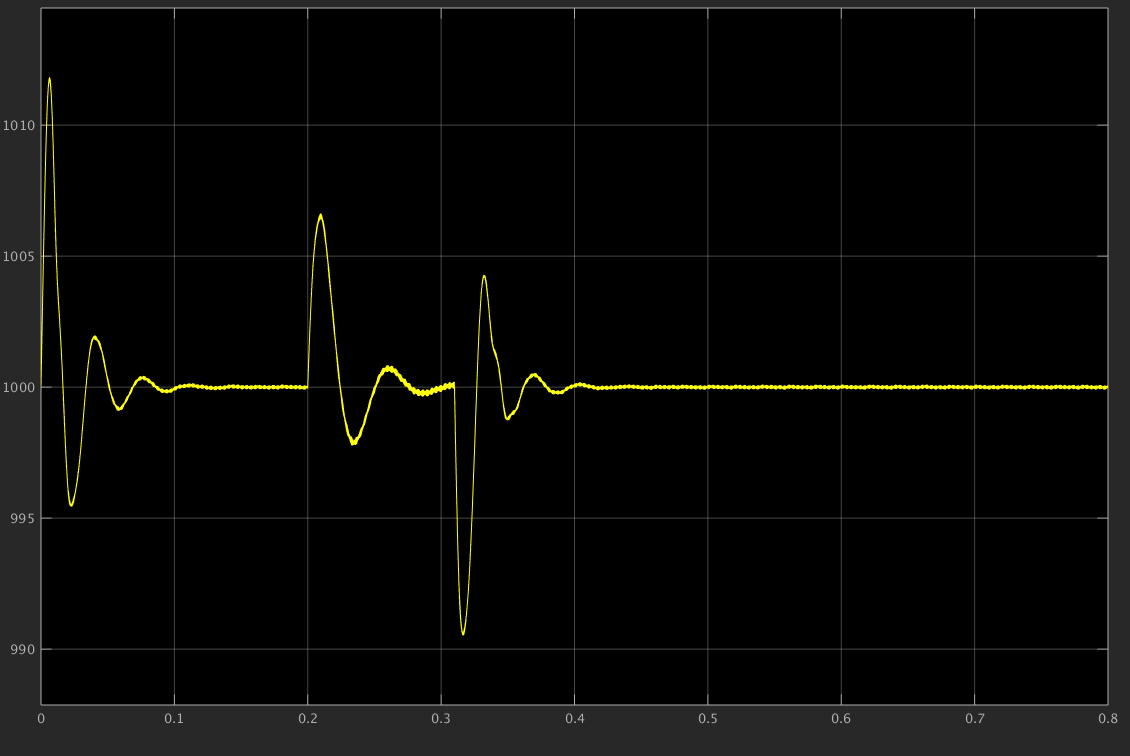
\includegraphics[width=.45\linewidth]{Images/bad1e6Sample_V_DC-side.png} }}%
      \qquad
      \subfloat[Sample time: 1e-7s]{{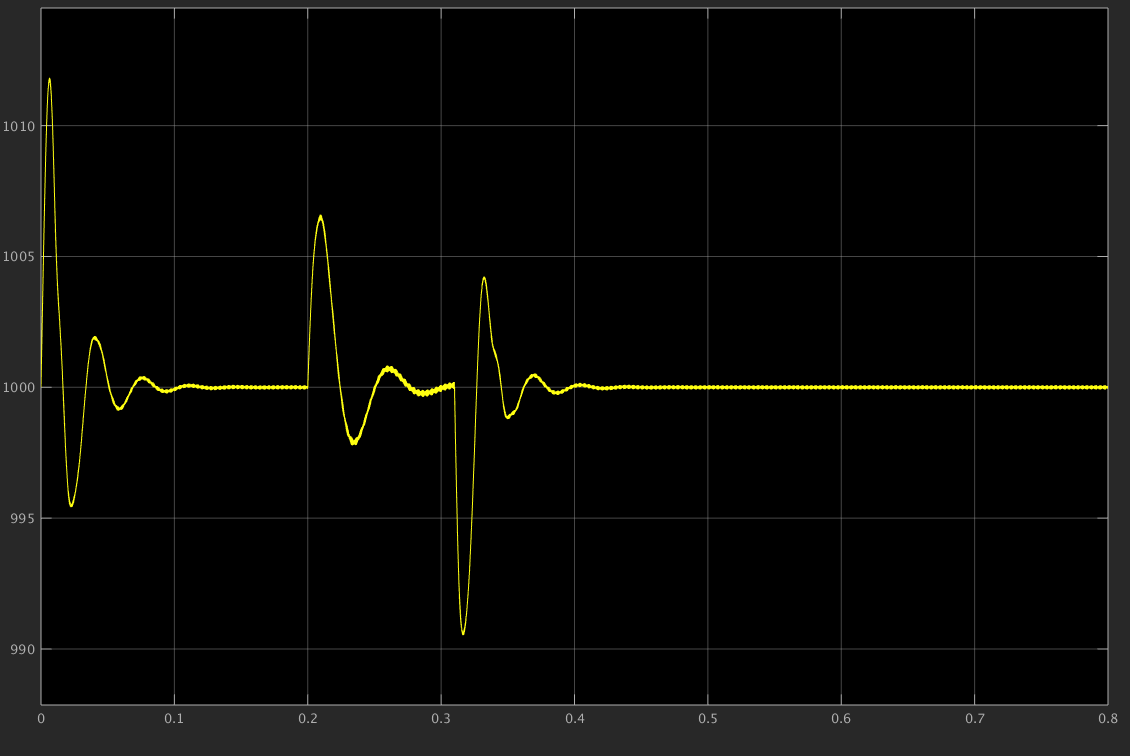
\includegraphics[width=.45\linewidth]{Images/1e7V_DC-side.png} }}%
      \caption{Simulation of the voltage read on the DC bus only changing simulation sample time}%
      \label{SampleTimeComp}%
  \end{figure}

  Finally, I decided to settle for the 1e-7s sample time given that I have enough memory and CPU power to avoid compromising the results.\\

  After the sample time issue was solved the PI controller was much simpler to adjust given that changes on the constants made actual logical sense.\\

\chapter{Power measuraments}

  Finally I added to the model a Simulink subsystem that measures the active and reactive power.

  \[ p(t)=v_d*i_d+v_q*i_q \]
  \[ q(t)=v_q*i_d-v_d*i_q \]

  \begin{figure}[H]
    \centering
    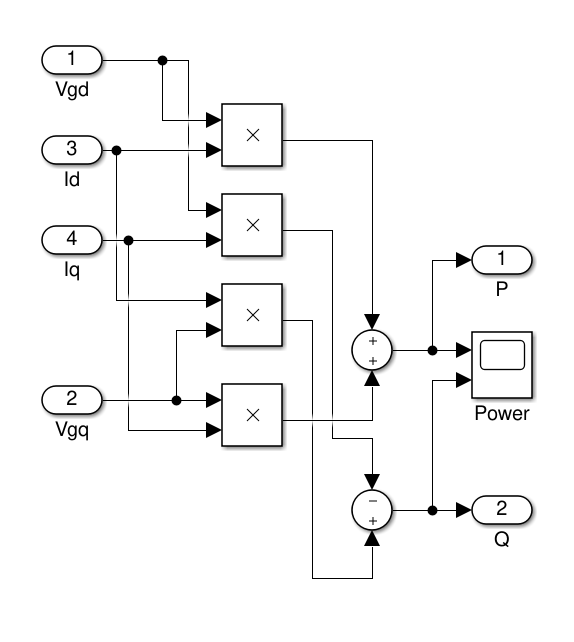
\includegraphics[width=.8\linewidth]{Images/PowerSubmodule.png}
    \caption{Power measurament submodule}
    \label{PowerSubmodule}
  \end{figure}
